%%
%% This is file `tikzposter-template.tex',
%% generated with the docstrip utility.
%%
%% The original source files were:
%%
%% tikzposter.dtx  (with options: `tikzposter-template.tex')
%%
%% This is a generated file.
%%
%% Copyright (C) 2014 by Pascal Richter, Elena Botoeva, Richard Barnard, and Dirk Surmann
%%
%% This file may be distributed and/or modified under the
%% conditions of the LaTeX Project Public License, either
%% version 2.0 of this license or (at your option) any later
%% version. The latest version of this license is in:
%%
%% http://www.latex-project.org/lppl.txt
%%
%% and version 2.0 or later is part of all distributions of
%% LaTeX version 2013/12/01 or later.
%%


\documentclass{tikzposter} %Options for format can be included here

\usepackage{todonotes}

\usepackage[tikz]{bclogo}
\usepackage{lipsum}
\usepackage{amsmath}

\usepackage{booktabs}
\usepackage{longtable}
\usepackage[absolute]{textpos}
\usepackage[it]{subfigure}
\usepackage{graphicx}
\usepackage{cmbright}
%\usepackage[default]{cantarell}
%\usepackage{avant}
%\usepackage[math]{iwona}
\usepackage[math]{kurier}
\usepackage[T1]{fontenc}


%% add your packages here
\usepackage{hyperref}
% for random text
\usepackage{lipsum}
\usepackage[english]{babel}
\usepackage[pangram]{blindtext}

\colorlet{backgroundcolor}{blue!10}

 % Title, Author, Institute
\title{Predict Future Sales}
\author{Siyu Chen}
\institute{ Xi'an Shiyou University, China \\
}
%\titlegraphic{logos/tulip-logo.eps}

%Choose Layout
\usetheme{Wave}

%\definebackgroundstyle{samplebackgroundstyle}{
%\draw[inner sep=0pt, line width=0pt, color=red, fill=backgroundcolor!30!black]
%(bottomleft) rectangle (topright);
%}
%
%\colorlet{backgroundcolor}{blue!10}

\begin{document}


\colorlet{blocktitlebgcolor}{blue!23}

 % Title block with title, author, logo, etc.
\maketitle

\begin{columns}
 % FIRST column
\column{0.5}% Width set relative to text width

%%%%%%%%%% -------------------------------------------------------------------- %%%%%%%%%%
 %\block{Main Objectives}{
%  	      	\begin{enumerate}
%  	      	\item Formalise research problem by extending \emph{outlying aspects mining}
%  	      	\item Proposed \emph{GOAM} algorithm is to solve research problem
%  	      	\item Utilise pruning strategies to reduce time complexity
%  	      	\end{enumerate}
%%  	      \end{minipage}
%}
%%%%%%%%%% -------------------------------------------------------------------- %%%%%%%%%%


%%%%%%%%%% -------------------------------------------------------------------- %%%%%%%%%%
\block{Introduction}{
    To predict total sales for every product and store in the next month. 
    Provided with daily historical sales data. The task is to forecast the total amount of products sold in every shop for the test set. Note that the list of shops and products slightly changes every month. Creating a robust model that can handle such situations.
     
  \vspace{.5cm}
  \centering

  \begin{tabular}{c|c} 
    \toprule
        % after \\: \hline or \cline{col1-col2} \cline{col3-col4} ...
        Fields  & Field to explain\\
    \midrule
    shop\_id & unique identifier for a store. \\
    item\_id & a unique identifier for a product. \\
    item\_category\_id  & a unique identifier for a category. \\
    item\_cnt\_day & quantity of products sold. \\
    item\_price & the current price of the goods. \\
    date\_block\_num & a consecutive month. \\
    item\_name & product name. \\
    shop\_name & shop name. \\
       \bottomrule
  \end{tabular}
  \vspace{.2cm}
  
}

%%%%%%%%%% -------------------------------------------------------------------- %%%%%%%%%%


%%%%%%%%%% -------------------------------------------------------------------- %%%%%%%%%%
\block{Data Processing}{
\begin{itemize}
  \item Use only shop\_ID and item\_ID that appear in the test set.
  \item Use only data whose price is greater than 0.
  \item Delete the unwanted columns, aggregate them monthly, and get a new data set.
  \item Remove outliers.
  \item Drop the text features.
\end{itemize}


}
%%%%%%%%%% -------------------------------------------------------------------- %%%%%%%%%%


%%%%%%%%%% -------------------------------------------------------------------- %%%%%%%%%%

%\note{Note with default behavior}

%\note[targetoffsetx=12cm, targetoffsety=-1cm, angle=20, rotate=25]
%{Note \\ offset and rotated}

 % First column - second block


%%%%%%%%%% -------------------------------------------------------------------- %%%%%%%%%%
\block{Data Visualization}{
    
    \item Draw line graph of average monthly sales and total monthly sales, average monthly sales were rising and peaking in December.

\begin{tikzfigure}%[Overall architecture of \emph{GOAM} algorithm]
     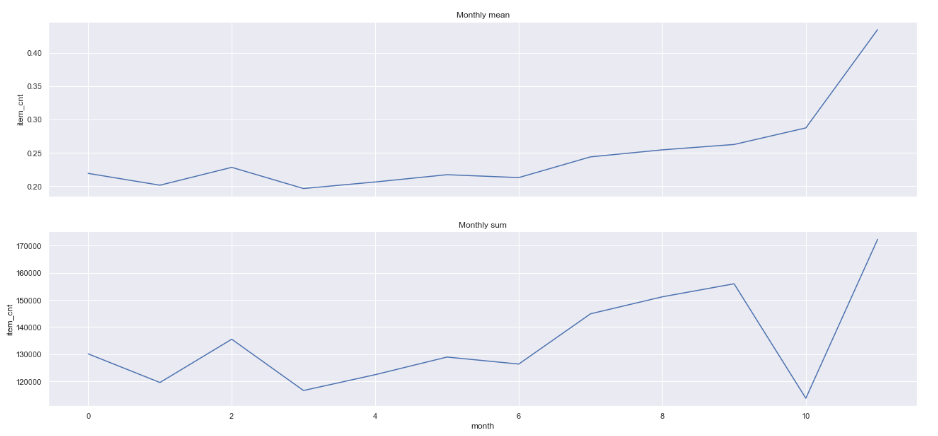
\includegraphics[width=0.6\linewidth]{figures/line.png}
        
    \end{tikzfigure}
    
        \item By visualizing by category, category 30 sells best, and only a few items sell well.
    
        \item Grouping by store number, most stores sell about the same, with only three doing particularly well.
    
        %   1) Group Feature Extraction,
%    2) Outlying Degree Scoring, and
%    3) Outlying Aspects Identification.

\begin{center}
    \begin{minipage}{0.8\linewidth}
    \centering
    \begin{tikzfigure}%[Overall architecture of \emph{GOAM} algorithm]
        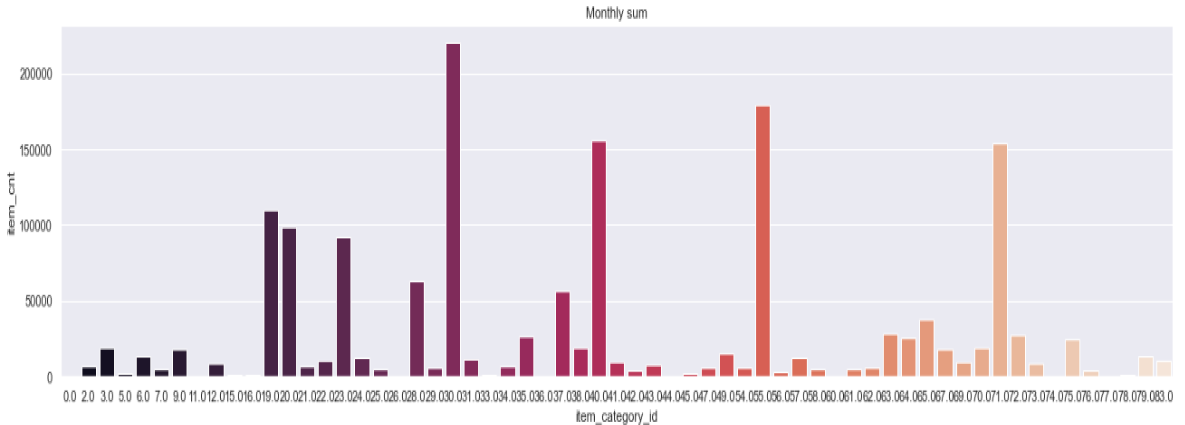
\includegraphics[width=0.8\linewidth]{figures/catg.png}
    
       \end{tikzfigure}%
       {\small{Grouping by category}}
    \end{minipage}
    \hfill
    \begin{minipage}{0.8\linewidth}
        \centering
        \begin{tikzfigure}%[Overall architecture of \emph{GOAM} algorithm]
            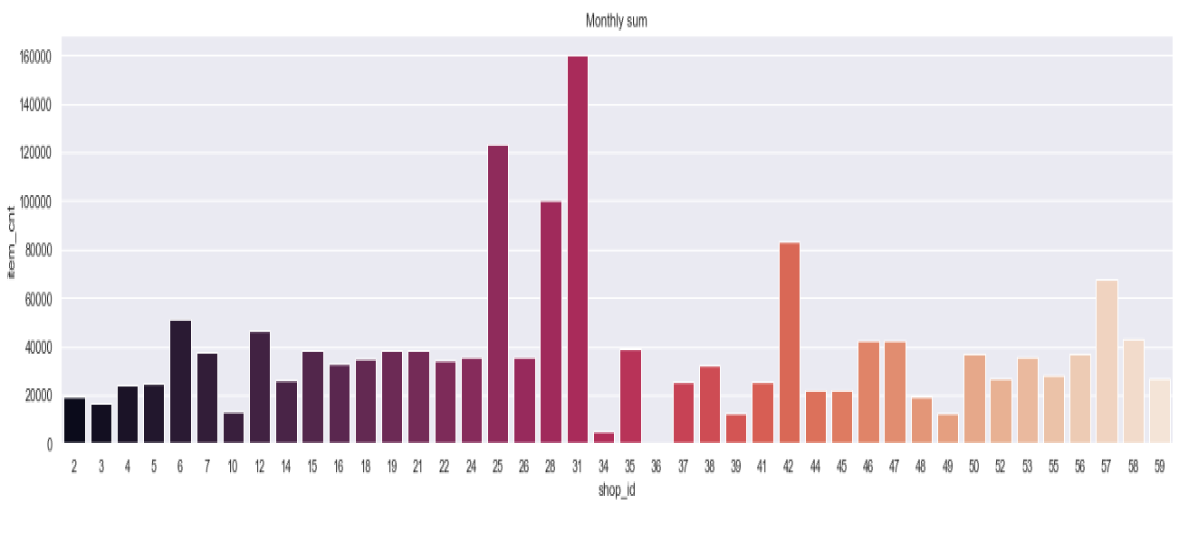
\includegraphics[width=0.8\linewidth]{figures/shop.png}
        
           \end{tikzfigure}%
           {\small{Grouping by shop\_id}}
        \end{minipage}
    
\end{center}

}
%%%%%%%%%% -------------------------------------------------------------------- %%%%%%%%%%


% SECOND column
\column{0.5}
 %Second column with first block's top edge aligned with with previous column's top.

%%%%%%%%%% -------------------------------------------------------------------- %%%%%%%%%%
\block{Feature Engineering}{

    \begin{itemize}
    \item
    The first 3-27 blocks are used for training.
    \item
    the five blocks 28-32 are used for verification.
    \item
    test set will be block 33 and our predictions should reflect block 34 values.
    \item
    Mean Encoding:
    \begin{itemize}
        \item
        Find the average monthly sales volume by store number.
        
        \item
        Find the average monthly sales volume by commodity number group.
        \item
        Find the average monthly sales volume of each item in each store.
        \item
        Group by year, find the average annual sales.
        \item
        Group by month, find the average monthly sales.
        \end{itemize}
\end{itemize}

}
%%%%%%%%%% -------------------------------------------------------------------- %%%%%%%%%%
% Second column - first block


%%%%%%%%%% -------------------------------------------------------------------- %%%%%%%%%%
\block[titleleft]{Build Model}
{
    \begin{itemize}
        \item
        \smallskip
        linear Regression\\
        Train rmse: 0.7347132326333324\\
        Validation rmse: 0.7755311093532987
        \item
        \smallskip
        Random Forest\\
        Train rmse: 0.6985868322226099\\
        Validation rmse: 0.776123635046122
        \item
        \smallskip
        XGBoost\\
        Train rmse: 0.697475453300762\\
Validation rmse: 0.798117433161014
    \end{itemize}
    XGBoost feature importance.
    \begin{center}
        \begin{minipage}{0.5\linewidth}
        \centering
        \begin{tikzfigure}%[Overall architecture of \emph{GOAM} algorithm]
            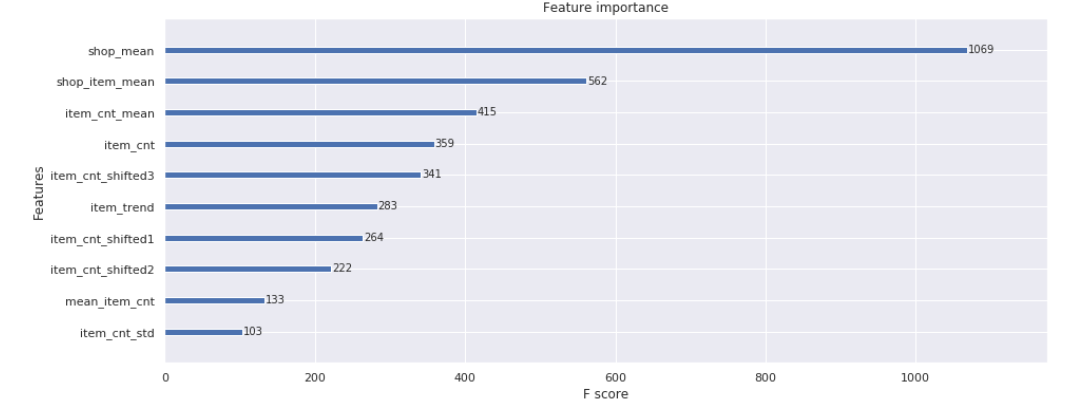
\includegraphics[width=1.0\linewidth]{figures/importance.png}
        
           \end{tikzfigure}%
           {\small{Feature importance}}
        \end{minipage}
        \hfill
        
        
    \end{center}
    
    Output the predictions of the first level model.

\vspace{.5cm}
\centering
\begin{tabular}{ c | c | c | c }
    \toprule
    &  random\_forest    & linear\_regression &xgboost\\
    \toprule
    0 &  0.98   &  0.85  &0.44   \\
    
    1 &  0.06   &  0.06 &0.10\\
    
    2 &   0.85   &  1.79 &0.50\\
    3 &   0.00   &  0.06 &0.10\\
    4 &   0.06   &  0.06 &0.10\\
    \bottomrule
\end{tabular}
           

}
%%%%%%%%%% -------------------------------------------------------------------- %%%%%%%%%%


% Second column - second block
%%%%%%%%%% -------------------------------------------------------------------- %%%%%%%%%%
\block[titlewidthscale=1, bodywidthscale=1]
{Ensembling}
{
    
    \begin{itemize}

        \item
        \smallskip
        \large
        {To combine the 1st level model predictions,to use a simple linear regression. 

        \item
        Trained on validation set using the 1st level models predictions as features.
        
        Make predictions on test set using the 1st level models predictions as features.
        
        Train rmse: 0.7654489715389068
        \item
        Output Dataframe:
        }
        
    \end{itemize}
  
    
    \vspace{.5cm}
\centering
\begin{tabular}{ c | c | c }
    \toprule
    &  ID    & item\_cnt\_month      \\
    \midrule
    0 &  0  &  0.85     \\
    
    1 &  1   &  0.08 \\
    
    2 &   2   &  1.29 \\
    3 &   3  &  0.06 \\
    4 &   4   &  0.08 \\
    5 &  5   &  0.96 \\
    6 &  6  &  1.25 \\
    7 &  7   &  0.21 \\
    8 &  8   &  1.99 \\
    9 &  9   &  0.06 \\
    \bottomrule
\end{tabular}
\begin{itemize}
    \item 
    \item 
    
\end{itemize}


}
%%%%%%%%%% -------------------------------------------------------------------- %%%%%%%%%%


% Bottomblock
%%%%%%%%%% -------------------------------------------------------------------- %%%%%%%%%%


%\note[targetoffsetx=8cm, targetoffsety=-10cm,rotate=0,angle=180,radius=8cm,width=.46\textwidth,innersep=.1cm]{
%Acknowledgement
%}

%\block[titlewidthscale=0.9, bodywidthscale=0.9]
%{Acknowledgement}{
%}
%%%%%%%%%% -------------------------------------------------------------------- %%%%%%%%%%

\end{columns}


%%%%%%%%%% -------------------------------------------------------------------- %%%%%%%%%%
%[titleleft, titleoffsetx=2em, titleoffsety=1em, bodyoffsetx=2em,%
%roundedcorners=10, linewidth=0mm, titlewidthscale=0.7,%
%bodywidthscale=0.9, titlecenter]

%\colorlet{noteframecolor}{blue!20}
\colorlet{notebgcolor}{blue!20}
\colorlet{notefrcolor}{blue!20}
\note[targetoffsetx=-13cm, targetoffsety=-12cm,rotate=0,angle=180,radius=8cm,width=.96\textwidth,innersep=.4cm]
{
\begin{minipage}{0.3\linewidth}
\centering

\includegraphics[width=24cm]{logos/tulip-wordmark.eps}
\end{minipage}
\begin{minipage}{0.7\linewidth}
{ \centering
Predict Future Sales,
  16/10/2020, xi'an, China
}
\end{minipage}
}
%%%%%%%%%% -------------------------------------------------------------------- %%%%%%%%%%


\end{document}

%\endinput
%%
%% End of file `tikzposter-template.tex'.
